% \iffalse
\documentclass[journal,12pt,twocolumn]{IEEEtran}
\usepackage{cite}
\usepackage{amsmath,amssymb,amsfonts,amsthm}
\usepackage{algorithmic}
\usepackage{graphicx}
\usepackage{textcomp}
\usepackage{xcolor}
\usepackage{txfonts}
\usepackage{listings}
\usepackage{enumitem}
\usepackage{mathtools}
\usepackage{gensymb}
\usepackage{comment}
\usepackage[breaklinks=true]{hyperref}
\usepackage{tkz-euclide}
\usepackage{listings}
\usepackage{gvv}
\def\inputGnumericTable{}
\usepackage[latin1]{inputenc}
\usepackage{color}
\usepackage{array}
\usepackage{longtable}
\usepackage{calc}
\usepackage{multirow}
\usepackage{hhline}
\usepackage{ifthen}
\usepackage{lscape}
\usepackage{caption}

\newtheorem{theorem}{Theorem}[section]
\newtheorem{problem}{Problem}
\newtheorem{proposition}{Proposition}[section]
\newtheorem{lemma}{Lemma}[section]
\newtheorem{corollary}[theorem]{Corollary}
\newtheorem{example}{Example}[section]
\newtheorem{definition}[problem]{Definition}
\newcommand{\BEQA}{\begin{eqnarray}}
\newcommand{\EEQA}{\end{eqnarray}}
\newcommand{\define}{\stackrel{\triangle}{=}}
\theoremstyle{remark}
\newtheorem{rem}{Remark}
\begin{document}

\bibliographystyle{IEEEtran}
\vspace{3cm}

\title{GATE: CH - 34.2022}
\author{EE23BTECH11010 - Venkatesh D Bandawar $^{*}$% <-this % stops a space
}
\maketitle
% \newpage
\bigskip

% \renewcommand{\thefigure}{\theenumi}
% \renewcommand{\thetable}{\theenumi}

\textbf{Question:} A process described by the transfer function
\begin{align}
    G_p(s) = \frac{\brak{10s+1}}{\brak{5s+1}} \nonumber
\end{align}
is forced by a unit step input at time $t = 0$. The output value immediately after the unit step input (at $t = 0^+$) is ? \hfill(Gate 2022 CH 34)\\
\solution
\begin{table}[!h] 
\centering
\begin{tabular}{|c|c|c|}
\hline
    Parameter & Description & Value\\
    \hline
    $P(s)$ & Plant Transfer Function & $\frac{0.001}{s\brak{\frac{s}{0.5}+1}\brak{\frac{s}{100}+1}}$\\
    \hline
    $C(s)$ & Lag Compensator  & $\frac{100\brak{\frac{s}{10}+1}}{\frac{s}{0.1}+1}$\\
    \hline
    $T(s)$ & Loop gain  & $P(s) C(s)$ \\
    \hline
    $\omega$ & Angular Frequency & 3rad/s \\
    \hline
\end{tabular}

\caption{Given parameters}
\label{given parameters list.gate.2022.ch.34}
\end{table}
\begin{align}
    G_p(s) = \frac{Y(s)}{X(s)} &= \frac{\brak{10s+1}}{\brak{5s+1}}\\
    u(t) \system{\mathcal{L}} \frac{1}{s} \label{laplace transform of unit function 2022.ch.34}
\end{align}
From equation \eqref{laplace transform of unit function 2022.ch.34}:
\begin{align}
    Y(s) &= \frac{\brak{10s+1}}{s\brak{5s+1}}\\
    &= \frac{1}{s} + \frac{5}{5s+1}
\end{align}
Taking inverse laplace transformation, 
\begin{align}
    \frac{1}{s} &\mathrel{\substack{\mathcal{L}^{-1}\\\longleftrightarrow}} u(t)\\
    \frac{1}{s-c} &\mathrel{\substack{\mathcal{L}^{-1}\\\longleftrightarrow}} e^{ct} u(t)
\end{align}
\begin{align}
    y(t) &= {1 + e^{\frac{-t}{5}}}u(t)\\
    y(0^+) &= 2
\end{align}

\begin{figure}[!h] 
    \centering
    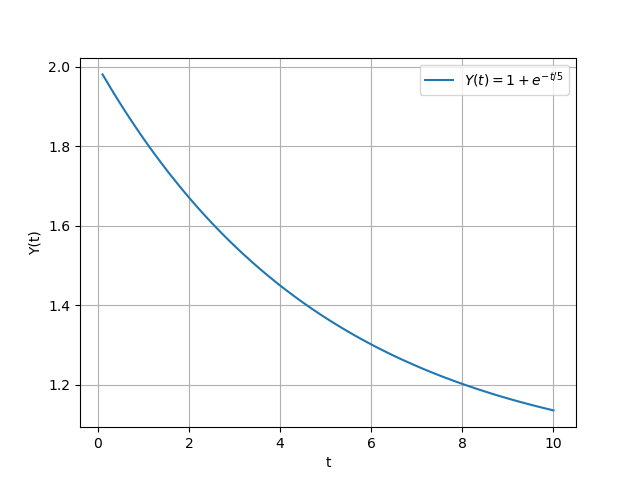
\includegraphics[width=\columnwidth]{figs/Graph_of_y(t).png}
    \caption{Graph of y(t)}
    \label{fig:Graph1_gate_CE_30}
    \end{figure}
\end{document}
